% !TeX program = xelatex
% (C) Hans Wan, Windy Deng
% Licensed under CC BY-NC-SA 4.0 International license.
% This is the LaTeX source code of Your Missing Semester of Using Computer (PDF Version).

\documentclass[a4paper]{book}
\usepackage{missing}

\date{\today}

\begin{document}

\pagenumbering{Alph}
\maketitle

\frontmatter
\pdfbookmark{内封}{innertitle}
\thispagestyle{empty}
\begin{center}
  \vspace*{2.5cm}
  \fontsize{42pt}{54pt}\selectfont{}\textsf{你缺失的那门}\par
  \fontsize{18pt}{18pt}\selectfont{}\textsf{Your Missing Semester of Using Computer}\par
  \fontsize{54pt}{8pt}\selectfont{}\textbf{\textsf{计算机课}}\par
  \vspace*{3.6cm}
\end{center}

\begin{note}
  本教程在持续更新之中,因此十分期望得到读者的建议和意见。
  无论是对编写方向有好的建议,还是发现了叙述不正确或不严谨的地方,亦或是找到了一个错别字,都请将反馈发送到邮箱 \href{mailto:missing@criwits.top}{missing@criwits.top}。
\end{note}

这是一份适合「电脑小白」的电脑使用技巧手册。
它以近乎「手把手教」的语言,介绍了从基本的文件管理到软件的寻找安装,从简要的硬件组成到电脑的安全防护,从小的使用技巧到优良软件推荐的许多内容,旨在帮助对电脑操作不甚了解的所谓「小白」逐渐上手电脑的使用。

\begin{center}
  \vspace*{1cm}
  
\includegraphics[width=5cm]{assets/QR_CODE.png}\par
  访问 \url{https://missing.criwits.top/} 或扫码阅读本教程的最新版本!\par
\end{center}  

\tableofcontents

\chapter{序}
\label{premble}

按理来说,对于所谓「Z 世代」的年轻人,熟练地使用电脑应该是他们的生活必备技能。

但事实却出乎我们意料。据我们观察,许多同学对电脑的使用也并不熟悉,甚至可以说是陌生:
他们可能在网上被下载到各种「P2P 高速下载器」,面对着满电脑的流氓软件而不知所措;
他们可能对着别人发来的 \texttt{zip} 或 \texttt{7z} 文件一头雾水,对「压缩」和「解压缩」都不甚熟悉;
他们可能装着四五个浏览器、三四个杀毒软件,更可能分不清自己电脑的「内存」和「硬盘」……

有人说,这是由于智能手机的普及造成的。
显然,使用电脑与使用手机相比,「复杂」了不止一个数量级;而随着智能手机的不断发展,人们借助一部手机就能完成许多事情,电脑似乎已经不再需要了。
可是,尽管几年前就有人说「电脑现在已经是夕阳产业了」,但事实却是:
至少在当下,我们仍然得学会去用电脑,不说多么「精通」,但至少要能知道「软件怎么找怎么装」「出现小问题怎么办」「XX 文件怎么打开」「怎么把文件打包」等等这些「21 世纪的常识」。

中小学的《信息技术》课堂、大学的《大学计算机基础》课程本应起到教授这些知识的作用。
可惜,事与愿违——很多时候,我们在这些课堂上学到的东西,可能一辈子都用不到;真正需要学的东西,却缺失了:

我们一辈子可能也不会再尝试用 Excel 排出张三李四不及格的科目有哪些,不会再折腾复杂到毫无意义的页眉和页脚,不会再碰和动画制作和网页相关的任何内容。
但我们未来必然有无数次会需要去网上下载一个新的软件,会无数次遇到各种各样的软件错误、闪退或者崩溃,会无数次因为 Windows 更新导致这样或那样的问题,会无数次遇到电脑沾上垃圾软件而奇慢无比无法使用……

这份《Your Missing Semester of Using Computer》是一份为「电脑小白」准备的电脑操作指南。
它直译过来就是《你缺失的那门计算机课》,也可以叫做《你本应学过的计算机课》。
我们会假定读者基本不了解电脑的操作,换言之就是所谓「电脑小白」,告诉读者「电脑最好怎么用」。

这份教程会在文中简称自己为《Missing》。
《Missing》的得名参考了 MIT 的《\href{https://missing.csail.mit.edu/}{The Missing Semester of Your CS Education}》。

\mainmatter

\part{基础篇}
\addtocontents{toc}{\protect\footnotetext[2]{标有「*」的为选读内容}}

\setcounter{chapter}{-1}

\chapter{一些约定与预备知识}
\label{first-things-first}

尽管《Missing》自认为受众是「电脑小白」,但我们依然不得不要求读者有一些最最基本的知识和操作经验。
此外,为了便于后续的讲述,我们会进行一些约定。

\section{容量与容量单位}

我们约定存储在电脑中的数据的容量单位「GB」「MB」「KB」等的关系如下:
\[1\,\mathrm{TB}=1024\,\mathrm{GB}=1024\times1024\,\mathrm{MB}=1024^3\,\mathrm{KB}=1024^4\,\text{字节}\]
即,我们统一使用「1024 进位」而不是「1000 进位」作为单位换算的系数。
此外,我们有时会略去这些单位最后的字母 B,即文中可能用「1 T」来表示「1 TB」。

你可能会问为什么要特别说明这里是「1024 进位」而不是「1000 进位」。
如果你有买过 U 盘,你会发现标称「128 GB」的 U 盘实际可用的容量只有 119 GB 左右。
这是因为生产 U 盘的厂家是用「1000 进位」来计算容量,而电脑自身是用「1024 进位」来计算容量的。
在这里我们进行容量单位的约定,是为了避免这种争议。

\section{文中的标记符号}

在《Missing》中,我们使用方头括号「【】」来标记所有屏幕上字面显示的选项。
例如,当我们希望你右键桌面上的图标
\begin{figure}[htb!]
  \centering
  
\includegraphics[width=2cm]{assets/This_PC.png}
\end{figure}

\noindent 时,我们会称「右键【此电脑】」。

我们使用右箭头「→」来表示下一步操作。
例如,「右键【此电脑】→【属性】」的意思是,右键桌面上的【此电脑】图标,然后在弹出的菜单中点击【属性】。

\section{快捷键的操作说明}

如果你按快捷键(多个键盘按键的组合键)后,电脑并没有行使理想中的功能,可能是你的按法不对。
快捷键的按法并不是「同时按下所有的键」,而是「依次序按下各键不松手,最后一起松开」。
例如,若要按快捷键「\keys{ + Shift + S}」:

\begin{itemize}
  \item 先按住 \keys{} 键(\keys{} 键上印有Window 徽标「」,一般来说这个键在 \keys{Ctrl} 和 \keys{Alt} 之间)不要松手;
  \item 再按住 \keys{Shift} 键,同样不要松手;
  \item 接着按一下 \keys{S} 键,然后松开全部按键。
\end{itemize}

\section{\keys{F1} -- \keys{F12} 功能键的使用说明}

对于笔记本电脑,其键盘最上方一排按键(\keys{F1} -- \keys{F12} 功能键)往往具有两重功能:
「它们本身的功能」和「它们的拓展功能」。

所谓「它们本身的功能」,指的就是 app 中规定的这些键的功能。
例如,在浏览器中,\keys{F5} 通常用来刷新页面,那么 \keys{F5} 键的「本身的功能」在浏览器中就是刷新页面。

所谓「它们的拓展功能」,指的是这些键上面画的图标所规定的额外功能。
例如,笔者的笔记本中 \keys{F5} 键上画有亮度降低的符号,因此 \keys{F5} 键的「拓展功能」就是降低屏幕亮度。

利用键盘左下角的 \keys{Fn} 键可以在这两种功能中切换。
具体地,对于一台电脑具有 \keys{Fn} 键设计的电脑,它可能是下列两种情况中的一种:

\begin{itemize}
  \item 直接按 \keys{F1} -- \keys{F12} 功能键可以行使它们本来的功能,按住 \keys{Fn} 的同时再按 \keys{F1} -- \keys{F12} 则行使它们的拓展功能。\\
    例如:如果 \keys{F5} 功能如上,那么,在这种情况下,按 \keys{F5} 可以在浏览器中刷新页面,按 \keys{Fn + F5} 可以降低屏幕亮度。
  \item 直接按 \keys{F1} -- \keys{F12} 功能键可以行使它们的拓展功能,按住 \keys{Fn} 的同时再按 \keys{F1} -- \keys{F12} 则行使它们本来的功能。\\
    例如:如果 \keys{F5} 功能如上,那么,在这种情况下,按 \keys{F5} 可以降低屏幕亮度,按 \keys{Fn + F5} 可以在浏览器中刷新页面。
\end{itemize}

你可以通过打开浏览器,打开某个页面,然后按 \keys{F5} 来测试你的电脑属于上面两种情况中的哪一种。
更一般地,用其他带有 \keys{F1} -- \keys{F12} 快捷键的软件来测试也是可以的。

很多笔记本电脑提供了一种快捷的方法在这两种模式中切换。
对于一些品牌的笔记本,你可以通过按 \keys{Fn + Esc} 来切换这两种模式。
另一些笔记本可能需要使用专门的软件(例如,Lenovo Vantage)或进入 BIOS 设置。
具体请查阅你设备的操作指南或自行上网搜索。

\section{有关「重启」的说明}

由于自 Windows 8 以来的 Windows 系统引入了「快速启动」的机制,现在「重启」这个过程并不等价于「先关机再开机」的过程。

故,若在文中提及「重启」这样的操作,请一定是选择开始菜单中的「重启」选项,而非点选「关机」后再手动打开电脑。

\practice

\begin{enumerate}
  \item 计算 1 GB 等于多少 KB?等于多少字节?假设一个汉字占两个字节,1 GB 大约可以记录多少个汉字?
  \item 尝试计算,一只按「1000 进位」计算得到容量为 64 GB 的 U 盘,它按「1024 进位」得到的容量是多少?
  \item 在自己电脑上尝试这些快捷键:
    \begin{enumerate}
      \item \keys{ + Shift + S} (仅限 Windows 10 / 11)
      \item \keys{Ctrl + Shift + Esc}
      \item \keys{ + D}
    \end{enumerate}
  \item 了解并试验自己笔记本电脑的 \keys{F1} -- \keys{F12} 功能键的拓展功能。
\end{enumerate}
\chapter{电脑以及电脑的组成}
\label{computer-and-its-components}

\begin{intro}
  在这一部分,我们将对「电脑」这种神奇的黑箱做一个简要的、整体的介绍。看完这一部分,你将可以找到这些问题的答案:

  \begin{itemize}
    \item 什么是「CPU」?他们说的「i5」「i7」都是什么?「双核」「四核」又是什么?
    \item 为什么说「内存和硬盘不一样」?为什么手机上我们都喊「内存」?电脑特别卡,到底是内存不够还是硬盘不够?
    \item 我想玩游戏,选购电脑时应该关注什么方面?
    \item 什么是「Windows」?那「Windows 10」又是什么?为什么那些用苹果笔记本的同学电脑界面看起来和我不一样?
  \end{itemize}
\end{intro}

电脑是由电路部分的硬件和电路之上的软件部分组成的。在大多数使用电脑的时候,我们都只与屏幕上的画面、窗口、文件打交道,但其实我们在使用过程中的许多问题都要牵涉到电脑的基本硬件设施。在本章,我们不妨先来看看电脑那内部几乎不为所见的「硬」的一面,之后再去看看为人所见却不甚了解的「软」的一面。

\section{电脑内部的硬件} 

这一节我们来介绍一台电脑内部的那些关键硬件。也许你并没有亲眼见过这些芯片和设备长什么样,但通过这一节的介绍,你应该能对它们有一个基本的了解。

\subsection{想象一个场景……}

我们先不谈硬件那些抽象的东西,我们假设这样一个场景:老师收了一个班的一摞作业,现在需要批改这些作业。

\begin{figure}[H]
  \centering
  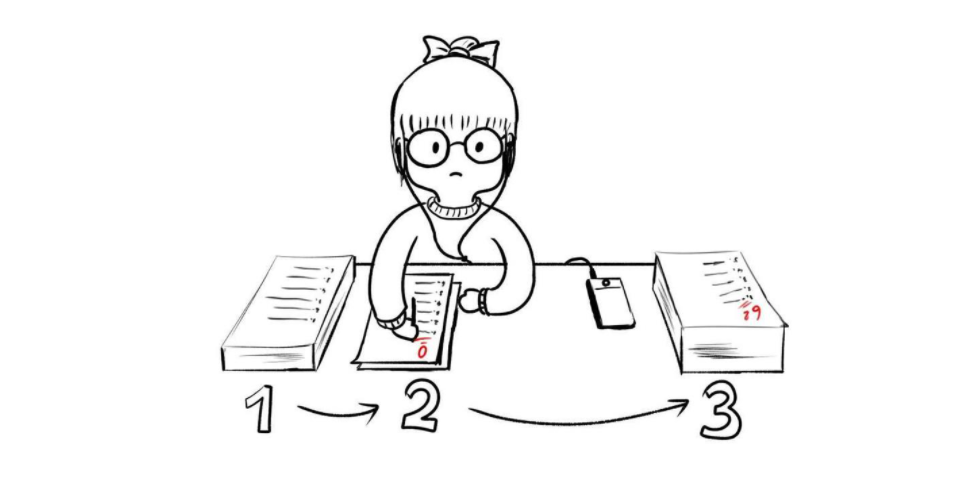
\includegraphics[width=7cm]{assets/Teacher_and_homework.png}
  \caption{老师和她需要批改的作业}
  \label{teacher-and-homework}
\end{figure}

老师批改作业的过程,可以简单地分解为下面这样几个步骤:

\begin{enumerate}
  \item 老师将这一摞作业堆在办公桌的一边,腾出办公桌的中央和另一边。
  \item 现在,老师取下这一摞作业中的一小叠,放在办公桌中央,开始伏案批改。
  \item 老师批改完了这一小叠作业,然后将它们放在办公桌的另一边,摞成新的一沓。
  \item 重复步骤 2 和步骤 3,最终老师完成了全部作业的批改,这时批改完的作业全部在在办公桌的另一边。
\end{enumerate}

我们会借助这个例子来更好地理解电脑硬件上的各个结构。

\subsection{处理器 / CPU}

中央处理器,简称「处理器」,英文简写「CPU」,是电脑内部最重要的一枚芯片,可以想象成是电脑的「大脑」。在上面的例子中,「老师」就相当于电脑中的处理器:「老师」的作用是对「作业」进行批改,从而完成教学任务;处理器的作用是进行各种的运算,从而实现电脑不同的功能。

你一定注意到过,电脑会发热——热到需要用一个风扇给它降温,这热量中有很大一部分就是处理器发出来的。如果你有关注过时事和新闻,中美贸易战中的「芯片」战,其中关键的一环就是处理器芯片。下图中,左为常见的台式电脑的 CPU 芯片,右为常见的笔记本电脑的 CPU 芯片。

\begin{figure}[H]
  \centering
  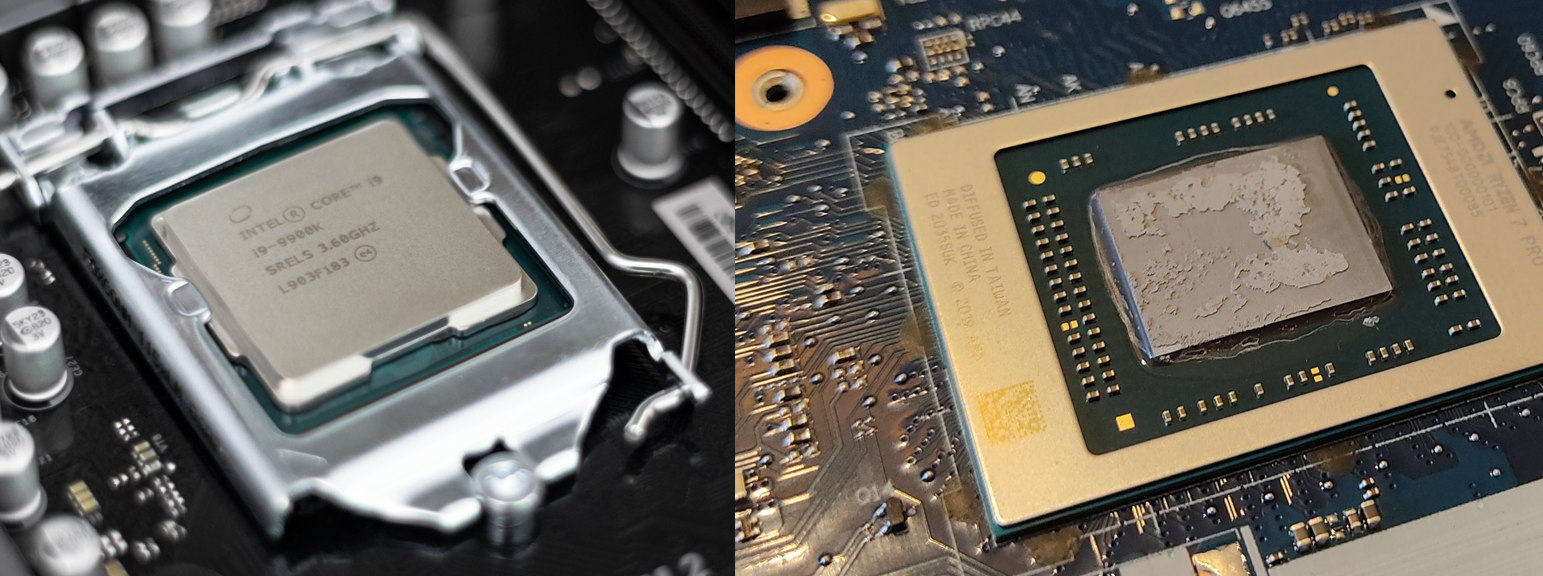
\includegraphics[width=10cm]{assets/CPUs.png}
  \caption{常见的台式机和笔记本电脑的处理器芯片。}
  \label{cpus}
\end{figure}

处理器是电脑工作的核心芯片,\regcolor{因此,处理器的性能就很大程度上决定了电脑的性能,决定了我们使用这台电脑流不流畅、玩游戏卡不卡、工作效率高不高}。在今天,全世界电脑芯片基本上是由两家美国公司设计制造\footnote{事实上,芯片的「设计」和「制造」两件事是不一样的,就像能设计出房屋的建筑师不一定会到工地上去砌墙。英特尔能够自行完成从设计到制造整条流水线,而 AMD 只能完成设计,它的处理器是由专门负责制造芯片的厂商(例如台积电)生产的。}的,其中一家叫做「英特尔」(Intel),另一家叫做「AMD」。

\begin{itemize}
  \item 英特尔公司现在主要的 CPU 产品线称作「酷睿」(Core),而「酷睿」系列又分成了 4 个档次——「i3」「i5」「i7」和「i9」。如果你现在在用笔记本电脑,不妨瞄一眼键盘下方是否有这样一个蓝色(也有可能是灰色,这里没有列出)的贴纸:
  \begin{figure}[H]
    \centering
    
\includegraphics[width=6cm]{assets/Stickers_Intel.png}
    \caption{英特尔的贴纸}
    \label{stickers-of-intel}
  \end{figure}
  \item AMD 公司现在主要的 CPU 产品线称作「锐龙」(Ryzen),而「锐龙」系列也分成了 3 个档次——「R5」「R7」和「R9」\footnote{其实还有 R3,但是很少在消费市场见到。}。如果你现在用笔记本电脑,不妨瞄一眼键盘下方是否有这样一个红色的贴纸:
  \begin{figure}[H]
    \centering
    
\includegraphics[width=2cm]{assets/Sticker_AMD.png}
    \caption{AMD 的贴纸}
    \label{sticker-of-amd}
  \end{figure}
\end{itemize}

我们常常说一个电脑是「双核」「四核」的,这里的「双核」「四核」也是处理器中的概念。这些处理器在一片芯片放了多个「核心」,相当于一个个协同起来的独立的小处理器。例如「双核」处理器,意味着在一枚处理器芯片上集成了两个核心,相当于两个大脑协同工作,当我们需要用电脑同时做很多事情的时候就有所裨益。同理,「四核」「八核」就是在一个芯片上集成了四个甚至是八个核心。

需要强调的是,\regcolor{并不是说核心数越多的处理器性能一定越好},更\regcolor{不是说 i7 处理器就一定比 i5 更好},也\regcolor{不是说英特尔的处理器就要比 AMD 好}。我们应该这样辩证地理解这些概念:每个品牌都有自己的不同系列,有的系列高端,有的系列低端;每个系列也都有自己的不同型号,有的型号性能强,有的型号性能弱。CPU 的性能并不与某一个因素呈线性的关系,而是多个因素综合的结果。

\subsection{内存 / RAM}

紧接着,我们介绍能直接与处理器交流的部件——内存,英文简写「RAM」。上一小节提到,处理器相当于大脑,但与大脑不同的是,处理器只能\regcolor{处理}数据,而这些待处理的数据,需要依赖外部的元件来临时存储。内存就是用来临时存储数据的。

内存本质也是一组芯片。生产内存这种芯片和生产处理器那种芯片所用的工艺有一些不同,目前生产内存这种芯片的厂商集中在韩国和中国台湾。一般这些芯片被排在条形的电路板上,这样的整体叫做「内存条」。下图中,上方的内存条是台式电脑使用的,下方的内存条是笔记本电脑使用的。

\begin{figure}[H]
  \centering
  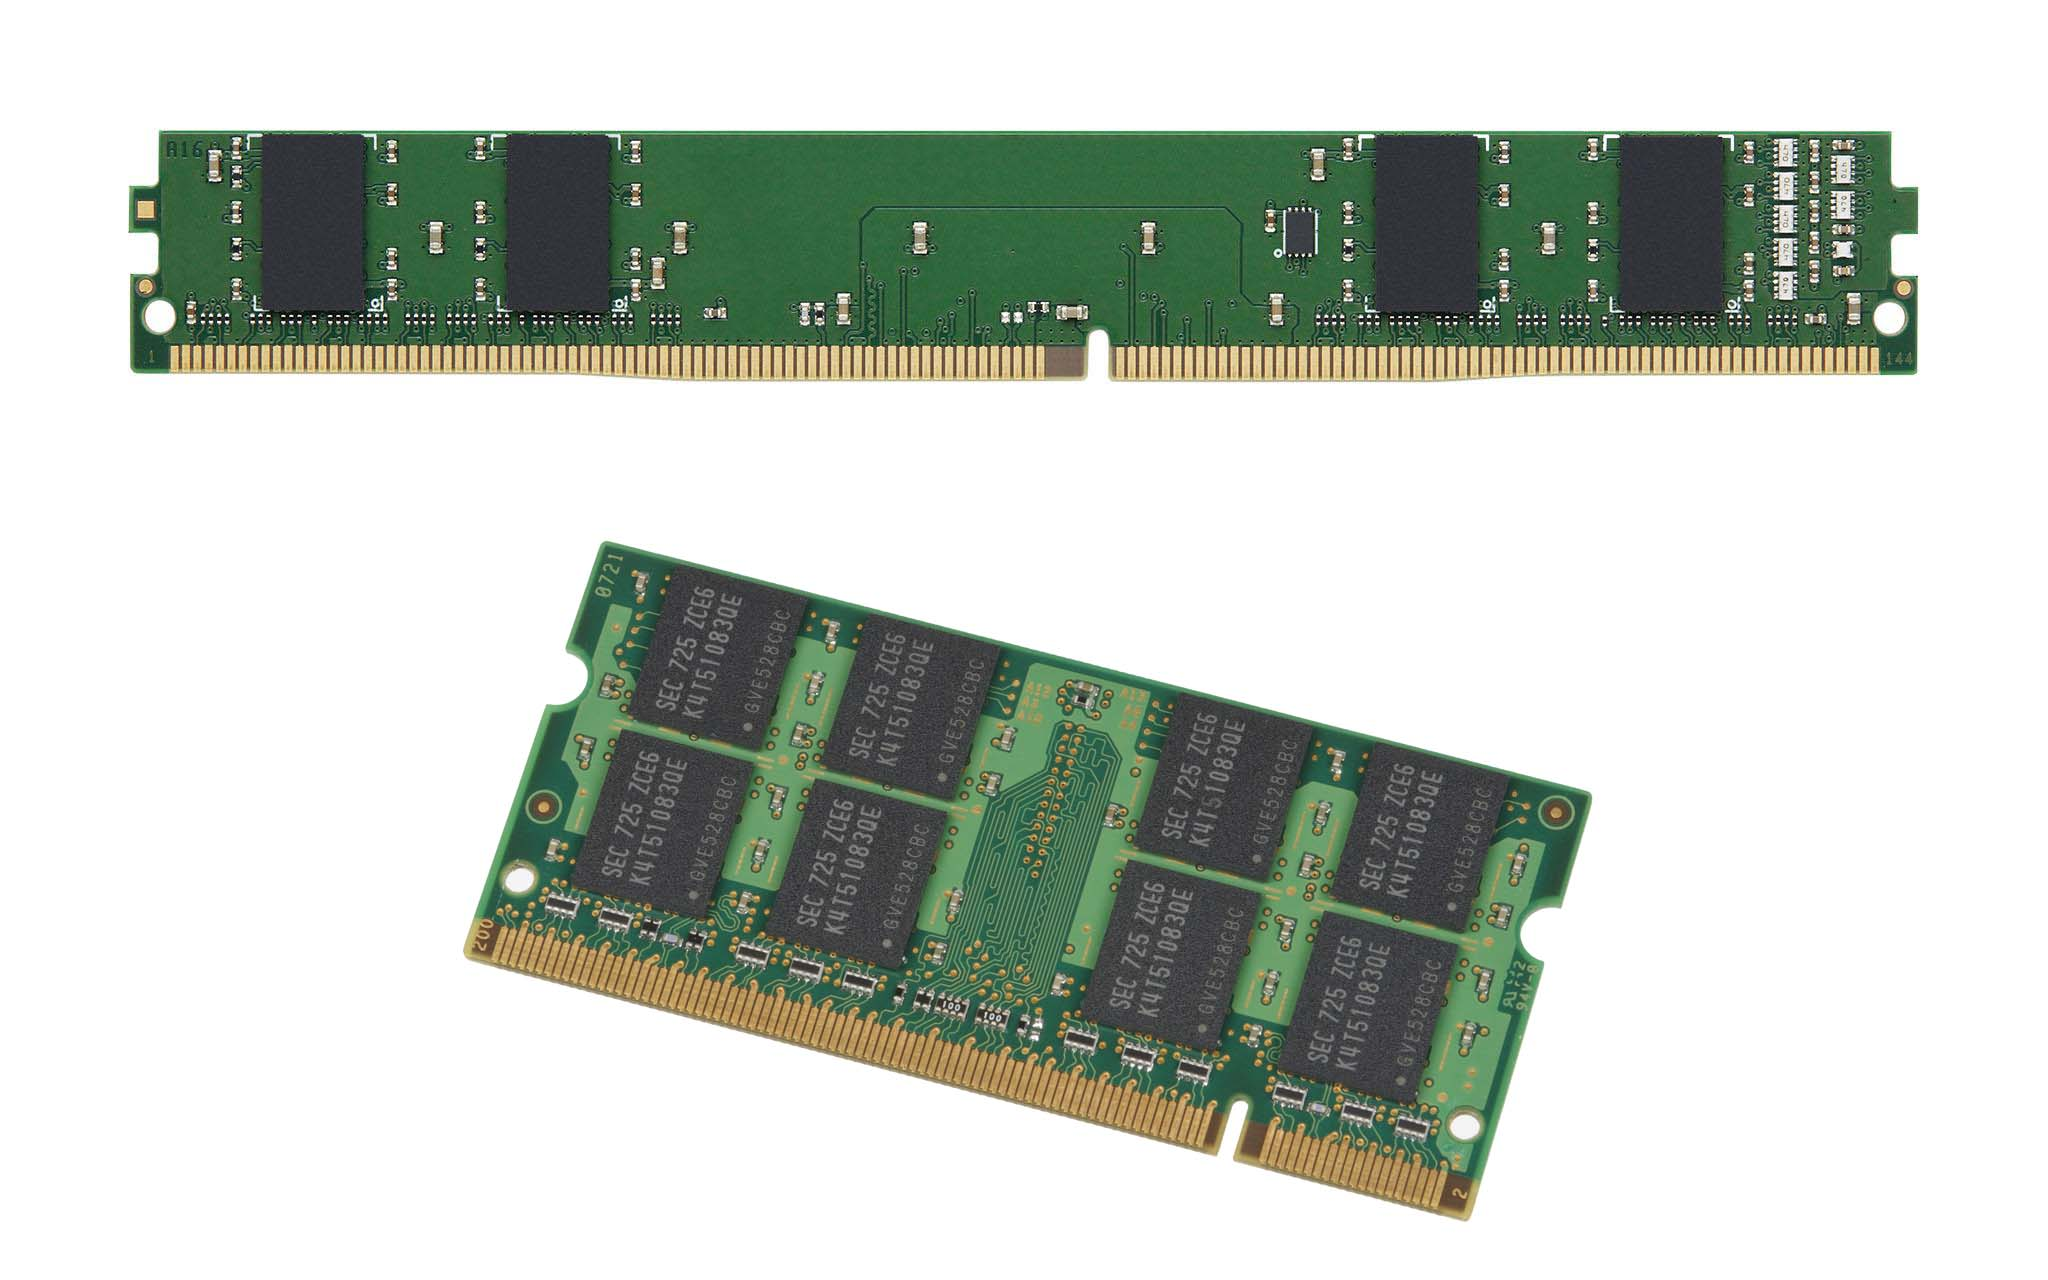
\includegraphics[width=8cm]{assets/RAMs.jpg}
  \caption{常见的内存条}
  \label{rams}
\end{figure}

前文说,内存直接与处理器进行数据交流。与处理器那极快的运算速度相匹配,内存的读取与写入速度也是极快的。但\regcolor{内存有一个特点——断电即丢失数据}。也就是说,当你电脑关机,内存中的数据便不复存在,又回到白纸一块。如果你想在内存里长久存放数据,那唯一的做法就是一直通电,多浪费电啊是吧。

回到前面老师批改作业的场景。办公桌的中央区域可以理解为「内存」:老师将作业放在办公桌中央批改,是因为这里改起来最方便;处理器将数据放在内存中处理,是因为这里读取和写入速度最快。办公桌中央不能总是放着东西,不然会弄乱、弄丢;内存中的数据一旦断电就会消失,因此总是临时的。

在 21 世纪初技术不是很发达的时候,内存的容量也不是很大,有 512 MB 已经不得了了。但随着时间的流逝,现如今大容量内存已经司空见惯。要想让现今的普通电脑基本流畅运行,内存容量应当至少有 4 GB。当然这东西倒是多多益善,就像更大的桌子能摆更多东西一样,\regcolor{更多的内存意味着更多的空间来让处理器存放数据,也就意味着电脑能同时处理更多的任务,基本意味着电脑更加流畅。}据我们的经验,流畅运行诸如 AutoCAD、Photoshop 之类的专业软件至少需要 8 GB 的内存。整体来说,在目前(2021 年),16 GB 的内存对于绝大多数人都已经够用了。

\begin{note}
  对应到手机中,内存有时会被手机厂商称为「运行内存」,不过我们不推荐如此称呼。
\end{note}

\subsection{硬盘}

内存是用来临时存储数据的,而硬盘则是用来长久保存数据的。与内存相比,硬盘的读写速度要慢得多,但存在硬盘中的数据不会因为断电而轻易消失,因此,\regcolor{硬盘是数据的最初的起点和最终的归宿}:处理器在一开始,从硬盘中取出数据放入内存,在内存中处理数据,处理完成之后,再将新的数据放回硬盘。

在前面老师批改作业的场景当中,办公桌两侧堆作业的地方可以理解为「硬盘」:大量的作业被堆在那里,整齐摆放,不会弄散、弄丢,但老师总是要把作业取到趁手的地方(办公桌中央)来批改;大量的数据被存在硬盘里,不会因为断电就丢失,但处理器总是要把数据放在快速的地方(内存)来处理。

简单来说,硬盘现在分为两种,一种叫「机械硬盘」(英文简称「HDD」)如下图左侧所示,一种叫「固态硬盘」(英文简称「SSD」)如下图右侧所。前者容量大、价格低、速度更慢,后者容量小、价格高、速度较快(但远远没有内存那么快)。前者是利用电磁原理存储数据,后者是芯片存储数据,但这种芯片和内存的那种又不一样——内存那种断电数据就消失了,固态硬盘的芯片断电还能保持数据。

\begin{figure}[H]
  \centering
  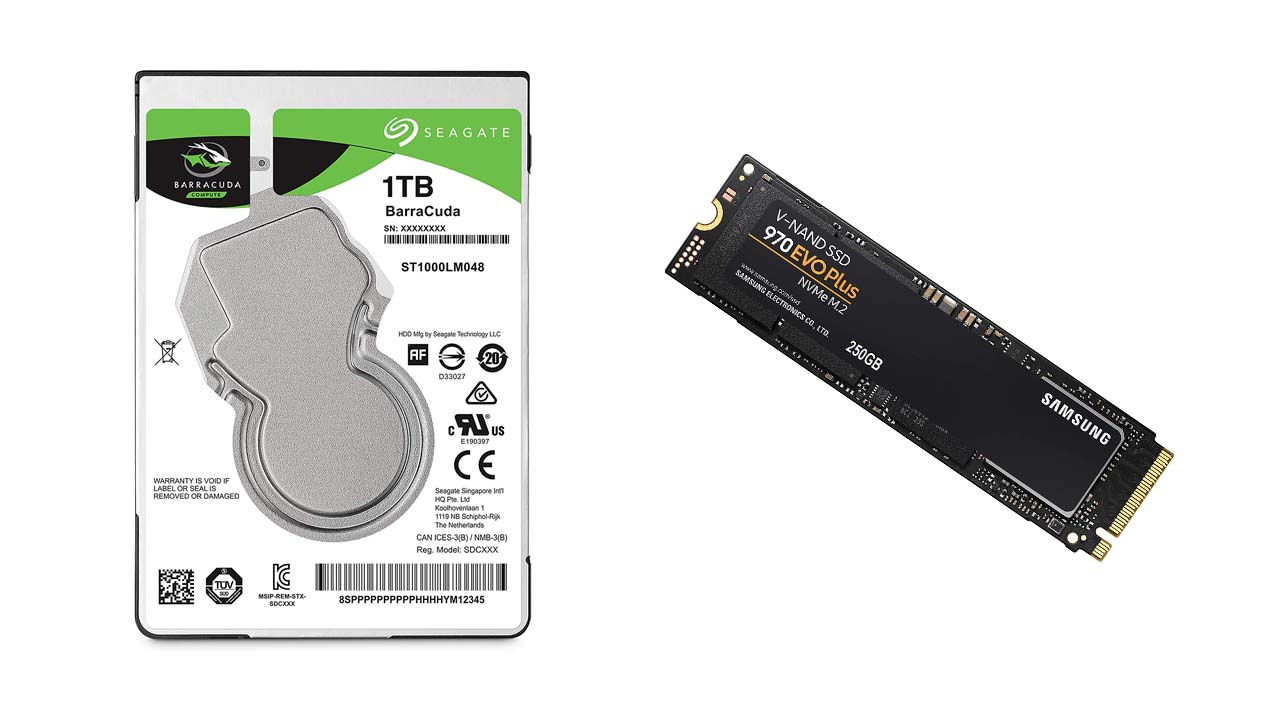
\includegraphics[width=8cm]{assets/Disks.jpg}
  \caption{常见的硬盘}
  \label{disks}
\end{figure}

在今天(2021 年),标称容量 512 GB 的固态硬盘大约 500 元,机械硬盘大约 200 元;标称容量 1 TB 的固态硬盘大约 800 元,机械硬盘大约 280 元。今天的中档次电脑常见的组合是用一块小容量(比如 256 GB)的固态硬盘,搭配一块大容量(比如 1 TB)的机械硬盘来实现各自功能的互补。稍微高档次一点的电脑,则会选用一整块更大容量(比如 512 GB 甚至 1 TB)的固态硬盘而不再使用机械硬盘。

打开桌面上的【此电脑】,你看到的所谓「C 盘」「D 盘」,就是硬盘上的空间——一块硬盘的空间可以被划分成不同的「盘」(学名叫「分区」)来更好地利用。

\begin{figure}[H]
  \centering
  
\includegraphics[width=10cm]{assets/Partition.png}
  \caption{打开【此电脑】,你就能看到硬盘的几个分区}
  \label{partitions}
\end{figure}


\regcolor{硬盘对电脑使用体验的影响,主要是「打开软件的速度」,包括「开机的速度」}。这是很容易理解的,因为数据原先都是存在硬盘里的,处理器从硬盘里「拿」数据的速度就直接影响着软件启动或者说加载的时间。

\begin{note}
  手机中也有类似固态硬盘一样的芯片来存储数据,它有时候被手机厂商称为「存储内存」,但它\regcolor{完全不是}内存。这是为什么有人会弄混「内存」和「硬盘」的根源之一。大家常说的「手机内存不够」,指的往往是存储空间(可以理解为「手机的硬盘」)不够,而不是真正的「内存」不够。
\end{note}

\subsection{显卡 / GPU*}

对于喜欢玩游戏的同学来说,「显卡」是他们在选购电脑时会着重考虑的一个因素。

最开始,「显卡」就是电脑里面的一个独立的芯片,像内存那样有自己的独立的电路板并插接在主板上。这个芯片的功能是专门进行画面的绘制和图像的处理,因而得名「显」卡。所有显示在屏幕上的画面,都是由显卡进行「绘制」的。因而\regcolor{显卡的性能主要是对游戏以及一些图形相关的工作(比如三维制图、视频剪辑)有较大影响}。下图是近 20 年前的电脑显卡的照片。

\begin{figure}[H]
  \centering
  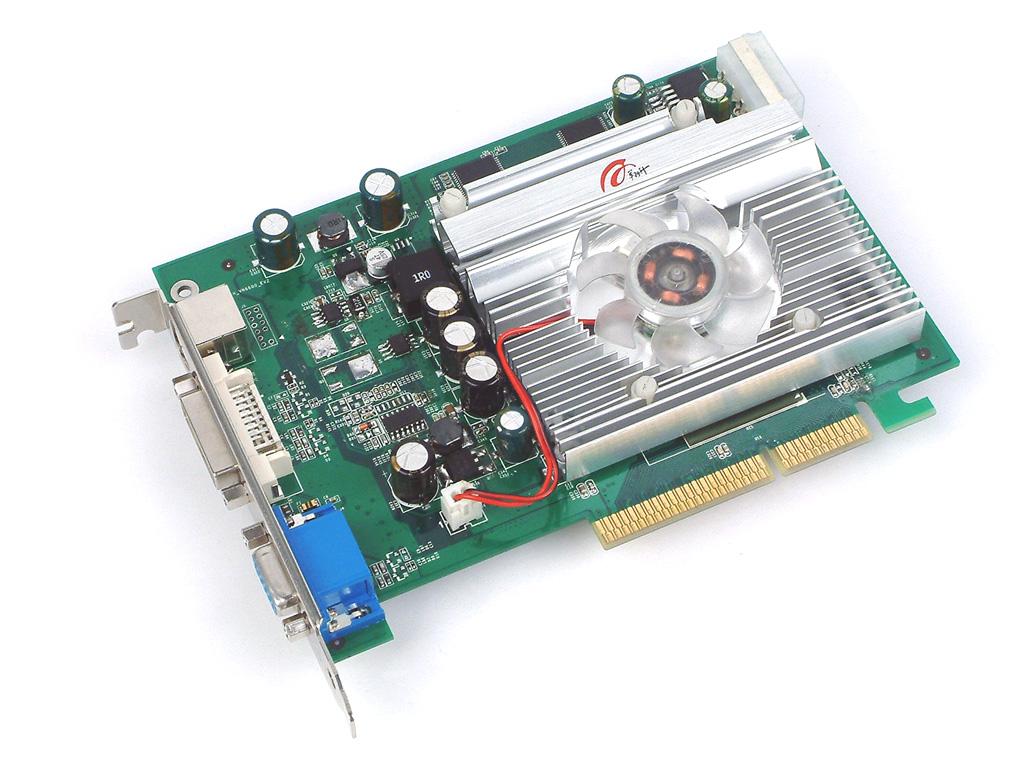
\includegraphics[width=8cm]{assets/Old_GPU.png}
  \caption{以前电脑上的显卡}
  \label{old-gpu}
\end{figure}

为什么上面那段要加上「最开始」三个字呢?因为随着半导体技术的发展,人们后来发现,显卡可以被「集成」到处理器\footnote{一开始,集成显卡并不是集成到处理器中的,而是集成在主板上的一个芯片之中(称为「北桥」),后来才集成到了处理器里面。}中,换言之,就像多核处理器把几个核心放在一个芯片上一样,显卡也可以和处理器放在一个芯片上。容易想到,这样集成到一起之后,显卡就不能做得很大了(受限于芯片整体的大小),也不能做得性能很强了(因为处理器核就在它边上,大家一起发热,一起分享能量),但可以缩小硬件的体积,也能降低功耗。因而,发展到今天,显卡在电脑中的形态有了以下两种:

\begin{itemize}
  \item \regcolor{集成显卡},英特尔称「核芯显卡」,AMD 称「APU」。显卡被安排在处理器的同一片芯片上,性能相对较差(但还是能应付大多数工作的,只是游戏、制图等特定工作就不太行了),功耗低,体积小。
  \item \regcolor{独立显卡},简称「独显」。显卡仍然是一片独立的芯片,有自己的供电和外围元件。这样的显卡性能比较强,但换来的是更高的功耗、更大的体积(游戏本为什么重)和更多的发热等。
\end{itemize}

\begin{figure}[H]
  \centering
  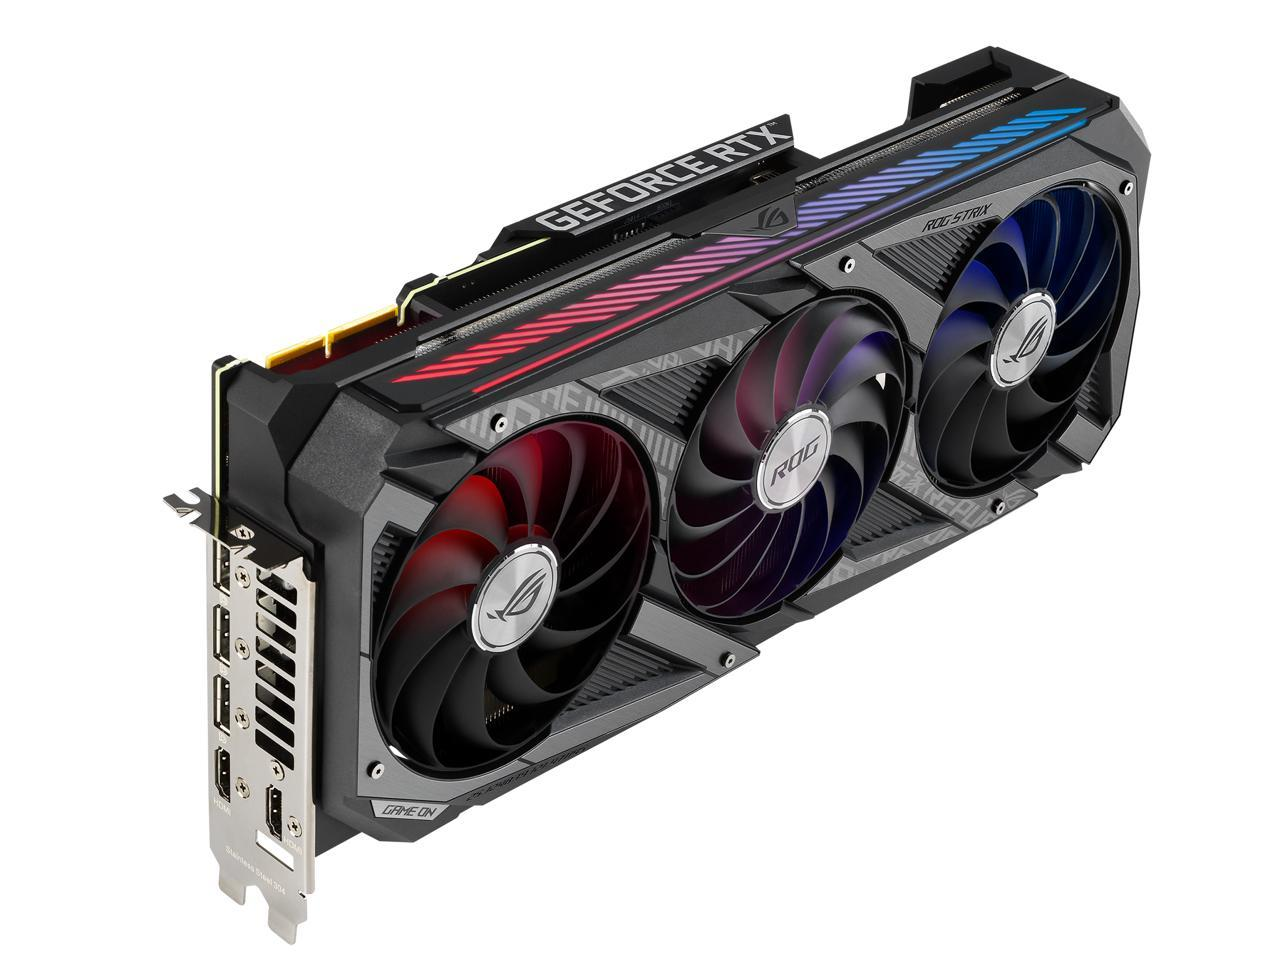
\includegraphics[width=8cm]{assets/3090.png}
  \caption{英伟达目前的顶级游戏显卡「RTX 3090」}
  \label{3090-gpu}
\end{figure}

今天,全世界生产\regcolor{独立显卡}的厂商主要有两家,一家叫「英伟达」(Nvidia),它生产的显卡俗称「N 卡」;另一家是前文提到过造处理器的「AMD」,它生产的显卡俗称「A 卡」。如果你有涉足过硬件交流圈,玩家所说的「RTX 3060」「GTX 1080 Ti」等都是英伟达显卡的型号,「RX 6800 XT」「RX 580」等都是 AMD 显卡的型号。上图是目前英伟达的顶级游戏显卡 RTX 3090。

\begin{note}
  是不是有人会问,那生产集成显卡的厂商有哪些呢?这个问题这里不回答,因为这不构成一个问题。
\end{note}


一般来说,对于笔记本,轻薄本都没有独立显卡而是使用集成显卡,游戏本都装配有独立显卡。这是由它们的使用场景和目标人群不同所决定的。

\section{与我们「打交道」的软件}

\subsection{软件与操作系统}

下面我们简单介绍「软件」和「操作系统」的概念。

由处理器、内存、硬盘以及各种各样的外围电子元件,共同构成了一台电脑的「硬件」部分。「硬件」就是电脑中电子电路的部分。而在「硬件」之上,硬件的具体工作任务是由「软件」来决定的。

我们用大家更熟悉的手机来做一个解释。\regcolor{手机上大家自己装的「QQ」「微信」「网易云音乐」,以及不是自己装的「电话」「短信」等 app 就属于「软件」}。「QQ」「微信」指导硬件去利用网络收发信息,利用屏幕展示数据,「网易云音乐」指导硬件去播放声音,同时在屏幕上展示评论,「电话」「短信」指导硬件利用无线电模块发送和接受信号……同样一部手机,硬件还是那个硬件,但能通过不同的软件行使不同的具体功能。

而在「QQ」「微信」「电话」等 app 之下,在纯粹的硬件之上,有\regcolor{一个更大、而且更「底层」的大软件,这个软件叫「操作系统」}。简单地说,操作系统「夹」在各个 app 和硬件之间,为 app 具体行使功能提供了一系列方便的「接口」。有了操作系统,网易云音乐的的开发者不再需要真正地去学习「怎么让喇叭发声」,而只需要学习「怎么告诉操作系统让喇叭发声」。「让喇叭发声」是一个带一些物理复杂知识的过程,但「告诉操作系统让喇叭发声」则相对简单得多。

\begin{figure}[H]
  \centering
  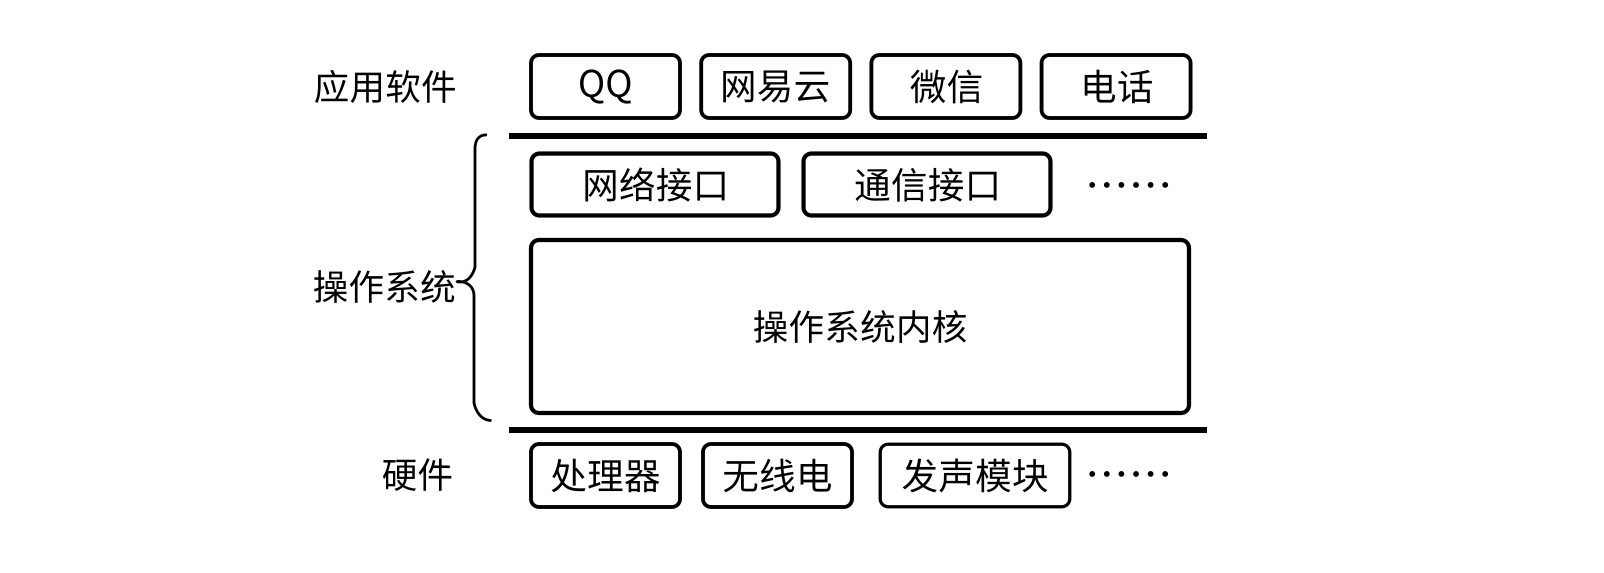
\includegraphics[width=10cm]{assets/Computer_Structure.png}
  \caption{App、操作系统和硬件的关系}
  \label{computer-structure}
\end{figure}

由于上层的软件(也就是 app)需要依赖操作系统来实现功能,而每个操作系统留给 app 的接口细节上有不同,因此,针对不同操作系统开发的软件是不能直接通用的。App 厂商一般会为不同的操作系统开发同一款 app,这样就能照顾到使用不同系统的用户。

今天主流的手机操作系统有「安卓」(Android)和「iOS」。后者只能使用在 Apple 的硬件上,前者则被各个手机厂商使用\footnote{华为开发的「鸿蒙」(Harmony OS)由于以某种方式兼容安卓软件,在这里我们暂且作为前者对待。}。而到了电脑上,「Windows」和「macOS」是最常见的两种操作系统。后者只能使用在 Apple 的硬件上。由于我们认为 macOS 的使用者不会依靠《Missing》来学习电脑知识,因而《Missing》中的所有操作都是认定读者使用 Windows 系统的。

下图中,左侧是 Windows 操作系统的典型界面,而右侧是 macOS 系统的典型界面。

\begin{figure}[H]
  \centering
  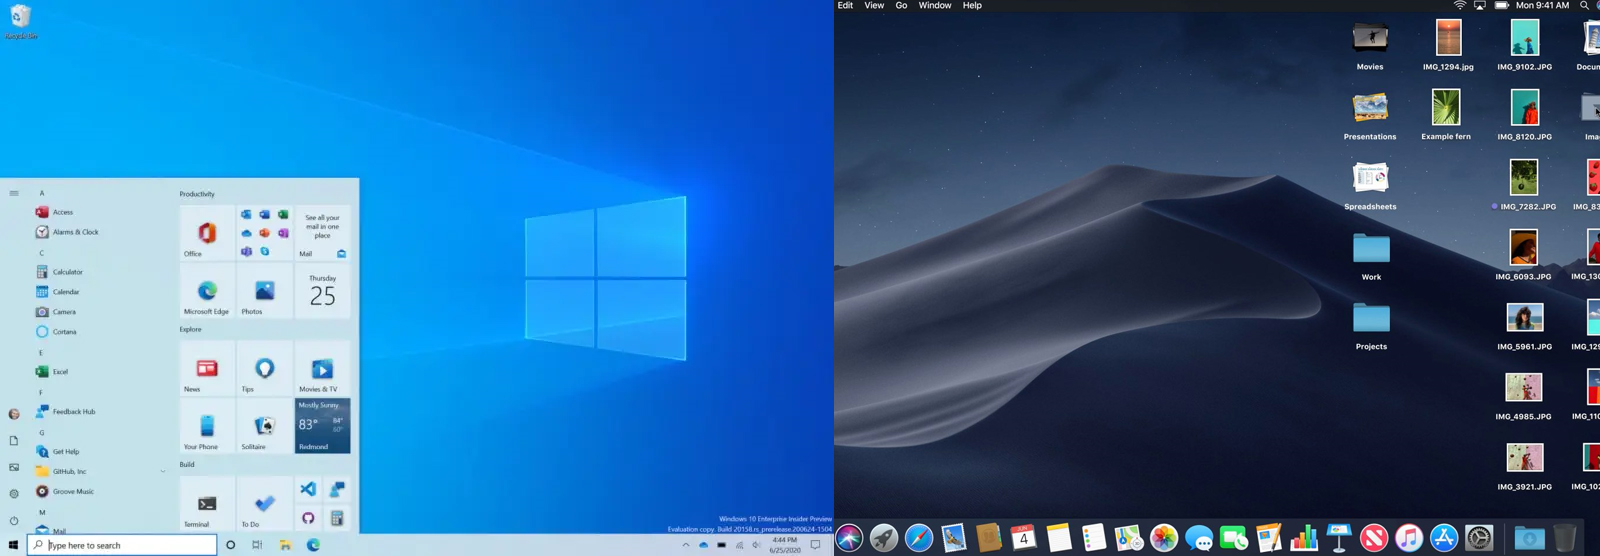
\includegraphics[width=10cm]{assets/Windows_and_macOS.png}
  \caption{Windows 和 macOS 系统的界面}
  \label{win-and-mac}
\end{figure}

\subsection{Windows 操作系统}

我们的大多数人使用的都是 Windows 操作系统。所谓「Windows XP」「Windows 7」和「Windows 10」则是 Windows 操作系统的不同版本。

Windows 由美国的微软公司(Microsoft)所开发,诞生于 1985 年。到今天(2021 年),Windows 已经经历了数个大版本的更新。目前最新的 Windows 版本是「Windows 11」(发布于 2021 年 10 月 5 日),我们大多数人使用的是「Windows 10」,还有一些稍旧的计算机在使用「Windows 7」。更老的 Windows 版本,例如「Windows XP」,已经鲜有使用。不同版本 Windows 系统之间会有操作细节、使用体验上的不同,不过往往最直观的不同是它们的「外观」。

Windows 可以使用在英特尔或者 AMD 处理器的电脑上——事实上,今天除了 Apple 以外几乎所有品牌的个人电脑都运行着 Windows 系统。通过右键桌面上的【此电脑】并点选【属性】,你可以看到自己电脑 Windows 系统的版本。

\begin{figure}[H]
  \centering
  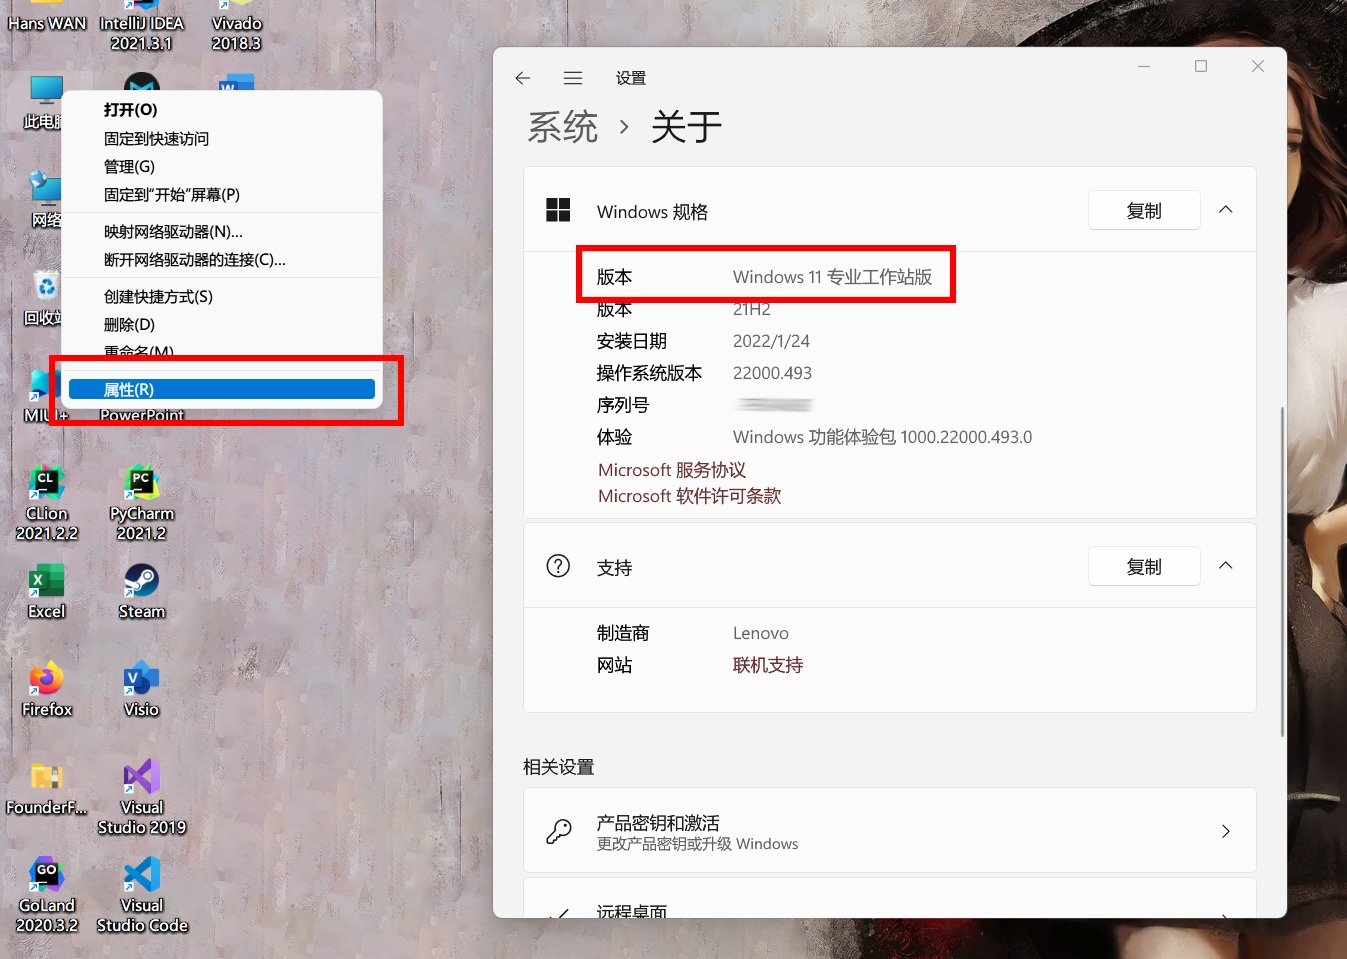
\includegraphics[width=8cm]{assets/Check_Windows_version.png}
  \caption{检查 Windows 系统的版本}
  \label{check-windows-version}
\end{figure}

《Missing》假定读者使用的系统是 Windows 10 或者 Windows 11,其中所有的操作都是基于 Windows 10 或者 Windows 11 简体中文版系统来描述的。如果你使用的是 Windows 7、Windows 8 或者 Windows 8.1,其中大多数操作也都能正常使用。一些明确仅能用于 Windows 10 和 / 或 Windows 11 的操作和技巧会被标注。

\practice

\begin{enumerate}
  \item 在之前打开的【此电脑】→【属性】,你除了能看到自己电脑的 Windows 版本之外,也能找到自己电脑的处理器型号和内存容量信息。尝试去查找这个信息,并自行上网搜索你的处理器型号,辨认它的品牌、系列,判断它是几核处理器,「主频」有多高。(「主频」是描述 CPU 性能的一个指标。)
  \item 你使用的是游戏本还是轻薄本?亦或是介于二者之间的所谓「全能本」?尝试翻到笔记本的底面,上网搜索它底面所写的型号,了解关于你自己机器的更多信息。
  \item 在 Windows 10 / 11 中,打开【任务管理器】,切换到【性能】选项卡,可以看到一个更详细的硬件运行状态,其中【硬盘】相关栏目展示了你设备的硬盘数量和类型(机械硬盘 HDD、固态硬盘 SSD)。尝试查看你电脑的硬盘容量和类型。
  
  你可以通过按 \keys{Ctrl} + \keys{Shift} + \keys{Esc} 来打开「任务管理器」。也可以右击【开始按钮】,选择【任务管理器】来打开它。
  \begin{figure}[H]
    \centering
    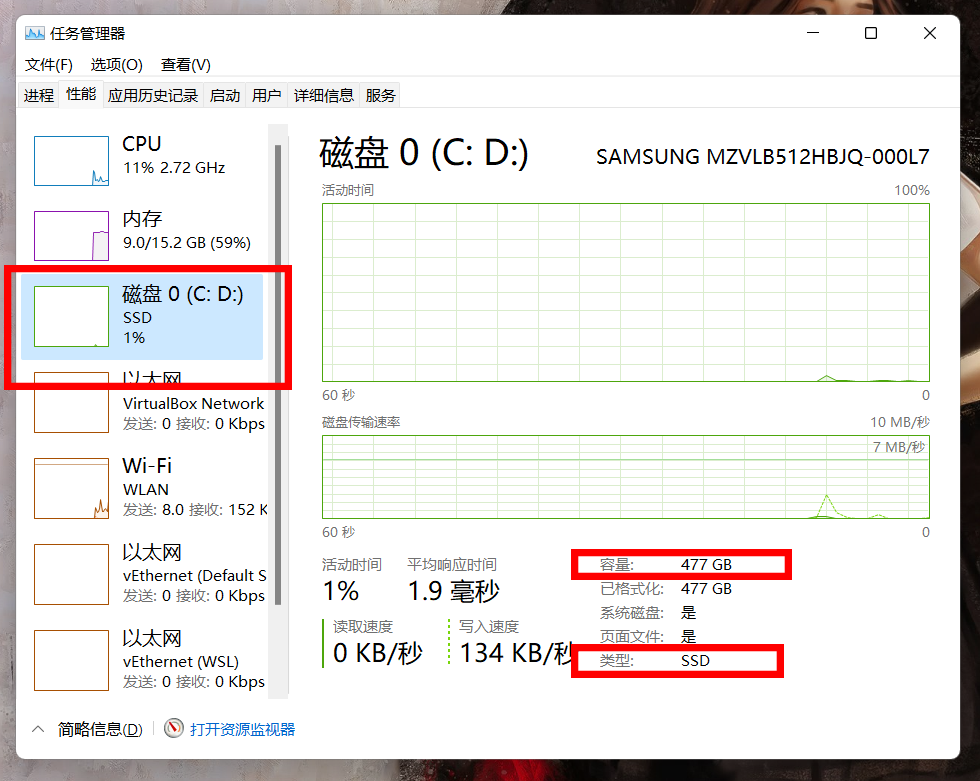
\includegraphics[width=8cm]{assets/Check_disk_status.png}
    \caption{查看电脑硬盘容量和类型}
    \label{check-disk}
  \end{figure}
  \item 你对「电路」的认知有多少?你是否好奇 CPU 是怎么运作的?从开关、导线、电池、灯泡组成的最简单「电路」到几乎无所不能「电脑」之间到底发生了什么奇妙的变化?《Missing》限于篇幅是不可能告诉你这些的。但是,你若有兴趣,可以去学习「电路电子技术」「数字电路与数字逻辑」「计算机体系结构」等相关内容。近年来,国际形势风云变幻,我国在芯片领域仍然存在许多短板。我们希望越来越多的有志青年能投身于包括但不限于体系结构、硬件组成、数字电路乃至微电子、半导体材料等领域,为我国芯片行业「补上短板」贡献自己的力量。
\end{enumerate}


\end{document}